\documentclass[letterpaper,10pt,prl,twocolumn,aps,reprint,superscriptaddress]{revtex4-1}
\usepackage{fullpage}
\usepackage{amsmath}
\usepackage{amsfonts}
\usepackage{amssymb}
\usepackage{graphicx}
% \usepackage{slashbox}
\usepackage{color}
\usepackage{longtable}
\usepackage{array}
\usepackage{dashrule}
\usepackage[shadow,colorinlistoftodos]{todonotes}

\newcommand{\comment}[1]{{\textbf{#1}}}
\newcommand{\cotwo}{CO$_2$ }
\newcommand{\COtwo}[1]{CO$_2$ }
\newcommand{\erf}{\text{erf}}
\newcommand{\bu}{\boldsymbol{u}}
\newcommand{\bx}{\boldsymbol{x}}
\newcommand{\bz}{\hat{\boldsymbol{z}}}
\newcommand{\grad}{\boldsymbol{\nabla}}
\newcommand{\cL}{\boldsymbol{\mathcal{L}}}
\newcommand{\cA}{\boldsymbol{\mathcal{A}}}
\newcommand{\cI}{\boldsymbol{\mathcal{I}}}

\newcommand{\prt}{\boldsymbol{\xi}}
\newcommand{\nrm}{{|\cdot|}}

\begin{document}

\title{A systematic method for the linear stability of an unsteady flow}
\author{Shreyas Mandre}
\affiliation{Brown University, Providence RI 02912 USA}
\author{Anja Slim}
\affiliation{Schlumberger-Doll Research Center, Cambridge MA 021?? USA}
\begin{abstract}
We look at solutal convection as a prototypical problem for linear stability of transient base states. 
We derive a formulation to determine the amplification of the most dangerous perturbation induced by the slowest growing norm. 
This formulation reduces to various classical and modern formulations of stability in special cases. 
We find that the threshold time for the growth of at least one perturbation in {\em every} norm (the onset of instability) agrees exactly with threshold found using frozen coefficient analysis. 
This formulation provides a rigorous justification for the frozen coefficient analysis to determine this threshold time.
\end{abstract}
\maketitle
% Background
\listoftodos
\vspace{1cm}

The study of solutal convection is motivated by carbon dioxide sequestration in deep aquifers\cite{SlimRama10,RapakaChen08,RiazHesse06,EnnisKingPreston05,EnnisKingPaterson05}. 
Super critical carbon dioxide introduced in the porous rock displaces the brine in the pores, rises to the top on account of being lighter than the brine, spreads horizontally along a cap rock, and starts dissolving in the brine. 
The solution of carbon dioxide in water is heavier than water, and therefore convection ensues as an instability of a diffusing (and hence transient) solute concentration gradient. 
\todo[inline]{How long before onset? The time scale for the convection is blah, which is sometimes as long as centuries. Do we have to wait for that long for convection to commence (finite time to onset) or does it commence immediately (zero time to onset).}
Instabilities of unsteady flows are frequently encountered on microscopic (the Richtmyer-Meshkov instability\cite{brouillette2002richtmyer}, foam mechanics \cite{anderson2010foam}) to geophysical scales (miscible viscous fingering\cite{homsy1987viscous}, transient shear flows leading to analogs of Kelvin-Helmholtz instability\cite{thorpe1968method}). 

% The problem with the state of the art
Linear stability analysis of such base flows is commonly performed by freezing the time-dependence of the base state, and examining the growth of perturbation around it using classical modal theories. 
This method, called the frozen coefficient analysis (a.k.a. quasi-steady analysis), is claimed to assume the base flow to evolve much slower than the growing perturbation. 
Therefore, the application of frozen coefficient analysis to determine the threshold of instability is considered inconsistent and met with skepticism because at the threshold the perturbations neither grow nor decay. 
While this discrepancy is widely acknowledged, the absence of an alternative formulation makes it difficult to evaluate the validity of the frozen coefficient analysis. 
The results from alternative methods based on quantifying the growth of a norm (e.g. L$_2$ norm) characterizing the size of the perturbation\cite{SlimRama10}, themselves depend sensitively on the choice of the norm, and are thus unable to resolve the inconsistency.

% Our resolution of the problem
In this letter, to address the sensitive dependence of the stability results on the choice of the norm, we extend the analysis to consider the slowest growing norm.
We find that this modification is equivalent to the classical modal analysis for steady base flows, Floquet analysis for time-periodic base flows, and the frozen coefficient analysis for characterizing the amplification of a perturbation for a short time since its inception. 
Using this modification, we show rigorously that a separation of time-scales is not required for the validity of frozen coefficient analysis, and that it gives the correct threshold for the onset of instability.
We demonstrate this result for a special case of the onset of solutal convection in porous medium.

\begin{figure}[b]
\vspace{5cm}
\caption{Schematic representation of the mathematical model.}
\label{fig:Schematic}
\end{figure}

% Mathematical model for solutal convection
We begin by introducing the mathematical formulation of the \cotwo convection problem.
Consider a semi-infinite layer of porous rock filled with supercritical \cotwo above a semi-infinite layer filled with brine, as shown in figure \ref{fig:Schematic}. 
We scale quantities such that the diffusivity of carbon dioxide, the Darcy mobility of the solution in the porous rock and the linear coefficient of buoyancy on \cotwo concentration is unity. 
At time $t=0$, the two layers come in contact and the \cotwo starts to dissolve and diffuse into the brine. 
The \cotwo concentration in the diffuse layer (scaled by the saturation concentration) is given by $C_0(z,t) = 1 + \erf( {z}/{2\sqrt{t}})$, where $z$ is the vertical coordinate, while the concentration in the \cotwo layer remains saturated and the fluid remains static. 
Perturbations about this state are governed by 
\begin{align}
 c_t + w C_{0,z} = \nabla^2 c \text{ and }
 \bu + \grad p + c\bz = 0
 \label{eqn:linone}
\end{align}
for $z<0$, and 
\begin{align}
 c = 0 \text{ and } \quad \bu + K (\grad p + c\bz) = 0
 \label{eqn:lintwo}
\end{align}
for $z>0$, where $c$ and $p$ are the perturbations in \cotwo concentration and pressure respectively, $\bu = (u,w)$ is the velocity, and $K$ is the ratio of mobilities in the supercritical \cotwo layer to that in the brine layer. 
We refer the reader elsewhere\cite{SlimRama10} for details. 

Formally, the linearization of governing equations for the dynamics of the perturbation $\prt$ about a transient base state leads to a non-autonomous system, written as ${d\prt}/{dt} = \cL(t)\prt$, where $\cL$ is the linearized operator. 
The system may be formally integrated $\prt (t_2) = \cA(t_2, t_1) \prt (t_1)$, where $\cA (t_2, t_1)$ is the propagator for the linear system from time $t_1$ to $t_2$. Solving the optimization problem 
\begin{align}
a_\nrm(t_2, t_1) = \max_{|\prt|=1} {| \cA(t_2, t_1) \prt|}, \label{eqn:amp1}
\end{align}
gives the amplification of a particular vector norm $|\cdot|$ induced by the dynamics on the most dangerous perturbation. 
Because of the time dependence of $\cL$, the amplification of the perturbation depends on both the inception time $t_1$ and the final time $t_2$, and all possible pairs $(t_1, t_2)$ must be considered. 
By choosing a suitable vector norm the amplification may be made arbitrarily large, even for the most benign $\cA$ (see supplementary material?). 
To ameliorate the dependence of amplification on the choice of the vector norm, we nest the optimization to find the vector norm which results in the least amplification as
\begin{align}
a(t_2, t_1) = \min_{|\cdot|} \max_{|\prt|=1} {| \cA(t_2, t_1) \prt|} = \min_{|\cdot|} a_\nrm (t_2, t_1). \label{eqn:amp2}
\end{align}
Defined thusly, $a$ is interpreted as the amplification of the most dangerous perturbation on the slowest growing (or least amplified) norm; 
if $a$ exists, every norm will exhibit an amplification of at least $a$ for its most dangerous perturbation.
\begin{figure}
 \centering
 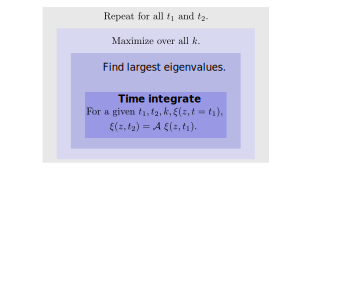
\includegraphics{./Figures/Algorithm}
 % Algorithm.pdf: 182x127 pixel, 72dpi, 6.42x4.48 cm, bb=0 0 182 127
 \caption{Schematic depiction of the nested algorithm used to find amplification $a(t_2, t_1)$ for the \cotwo convection problem. Each rectangle represents a subroutine performing the function listed in it, which is passed as a black-box to the nesting rectangle.}
 \label{fig:Algorithm}
\end{figure}

The solution to this optimization is possible owing to two theorems from finite-dimensional linear algebra, and yields the optimum to be the spectral radius $a(t_2,t_1) = \rho(\cA)$ of $\cA$. 
The first theorem states that for every vector norm $\rho(\cA) \le a(t_2,t_1)$, as can be easily verified by substituting the eigenvector corresponding to the largest magnitude eigenvalue of $\cA$ in \eqref{eqn:amp1}. 
The second theorem states that there exists a vector norm for which the spectral radius comes arbitrarily close to $a(t_2,t_1)$\cite{bulirsch2002introduction}; {\it i.e.} for at least one $\nrm$ and $\epsilon>0$, $\rho (\cA) + \epsilon > a(t_2,t_1)$. 
Combining the conclusions of the two theorems proves our claim that $a(t_2, t_1) = \rho(\cA)$. 
Instability ensues when $a(t_2, t_1) > 1$.
While the applicability of this conclusion is strictly valid for finite-dimensional systems, we believe that similar proofs should be possible for infinite-dimensional systems with only a few active modes ({\it e.g.} where diffusion damps out high wavenumbers, such as for \cotwo convection).

Using the spectral radius for amplification agrees exactly with classical methods in the case of autonomous and time-periodic linear systems. 
For autonomous systems, $\cA = \exp(\cL (t_2-t_1))$, and therefore $a(t_2,t_1) = \rho (\cA) = e^{\sigma (t_2-t_1)}$, where $\sigma$ is the largest real part of the eigenvalue of $\cL$. 
Thus, $a(t_1,t_1)>1$ if and only if Re($\sigma$)$>0$, which is the classical criterion for linear instability.
Similarly, for time-periodic systems with period $T$ restricted to $t_2 -t_1 = n T$ for some integer $n$, $a(t_2, t_1) = \rho (\cA ) = e^{n \beta T}$, where $\beta$ is the Floquet exponent with the largest real part. 
Again $a(t_2,t_1)>1$ implies Re($\beta$)$>0$, which is the classical criterion for instability of periodic systems using Floquet theory.

Tacit assumption about the linear space spanned by the perturbations. Should it be added? Do I understand it enough to claim so in a publication?

In this framework, the frozen coefficient analysis is considered applicable when $t_2 - t_1 \equiv \Delta t \ll 1$, and not in terms of a separation of timescales for the evolution of the perturbations compared to the background.
To illustrate this concept, we expand the propagator for small $\Delta t$ as $\cA = \cI + \Delta t \cL + \frac{1}{2} \left(\cL^2 + d\cL/dt \right) \Delta t^2 + \dots$, where $\cI$ is the identity operator. 
In this limit, $a(t_1 + \Delta t, t_1) = \rho(\cA) = 1 + \sigma(t_1) \Delta t + O(\Delta t^2)$, where $\sigma(t_1)$ is the largest real part of the eigenvalue of $\cL(t_1)$.
The threshold of instability in this framework ($a(t_2,t_1) = 1$) implies and is implied by $\sigma(t_1) = 0$ to $O(\Delta t)$, which agrees with the threshold criterion used by the frozen coefficient analysis.
This analysis demonstrated that frozen coefficient analysis predicts a necessary and sufficient condition for perturbations to grow for small times. It is also possible to demonstrate that $\sigma(t) < 0$ is a sufficient condition for perturbation decay in the general case using $\cA(t_3,t_1) = \cA (t_3, t_2) \cA(t_2, t_1)$. The inequality of the spectral radii of product of operators, $\rho(\cA(t_3,t_1)) \le \rho(\cA(t_3,t_2)) \rho(\cA(t_2,t_1))$, implies $a(t_3, t_1) \le a(t_3, t_2) a(t_2, t_1)$. Using this inequality, along with the aforementioned expansion of $\rho(\cA)$ for small $\Delta t$, it is elementary to prove that $da/dt < 0$ if $\sigma(t)<0$. Combined with the initial condition $a(t_1, t_1) = 1$ for all $t_1$, this analysis proves that $a(t_2, t_1)<1$ if $\sigma(t)<0$ for $t_1<t<t_2$, which is a sufficient condition for stability.

We now turn our attention to the case of \cotwo convection as an application of this method. 
Given the $x$-translational invariance of (\ref{eqn:linone}-\ref{eqn:lintwo}), we decompose the $c$, $p$ and $\bu$ in Fourier modes to exploit their independent evolution with time. 
The Fourier mode with wavenumber $k$ evolves according to
\begin{align}
 \text{insert equation(s) here}.
\end{align}
The determination of amplification according to \eqref{eqn:amp2} is found using a multiply nested algorithm shown schematically in figure \ref{fig:Algorithm}. 
Each rectangle represents a subroutine for performing the function listed inside it, and is passed as a black box to the rectangle immediately outside it.
The innermost level of this algorithm is the time-integrator, which takes the initial condition $\prt(z, t_1)$ of wavenumber $k$ and evolves it to a given future time $t_2$. 
This subroutine is used by an implicitly restarted Arnoldi algorithm for iteratively finding the largest magnitude eigenvalue implemented by the ARPACK package\cite{lehoucq1998arpack}. 
The parameters $t_1$, $t_2$, and $k$ are also passed to this subroutine. 
The eigenvalue calculation routine is in turn passed as a black box to an optimization algorithm based on the golden section method to find the most dangerous wavenumber. 
This routine finds the $k$ with maximum amplification for a given $t_1$ and $t_2$. 
Finally, this optimization is repeated for a range of $t_1$ and $t_2$. 
The execution of this algorithm results in an amplification of most dangerous perturbation on the slowest growing norm for each time pair $(t_1, t_2)$. 

Results
The only parameter in our problem is the ratio of mobilities $K$. \todo[inline]{Include discussion on the role of $K$ here.}
\todo[inline]{Explain a sample amplification heat map. Interpretation of neutral curve and other contours.}
\todo[inline]{Comparison with other norms. Demonstrate that other norms always show amplification larger than the spectral radius.}
\todo[inline]{Explain properties of the threshold. The neutral curve always intersects $t_1 = t_2$. The time of earliest growth (onset) is on the curve $t_1 = t_2$. The neutral curve emanates perpendicular to $t_1=t_2$, when eigenvalues are real. }
Interpretation

\vspace{1cm}

Even if the amplification is greater than unity, because the perturbation is assumed to be infinitesimal in magnitude, it is not possible to determine based on the linear amplification analysis alone whether the growing perturbation will visibly alter the system. 
Knowledge of the statistical distribution of spectrum of initial perturbations or the external influences feeding the perturbation is needed to make such a prediction in this framework. 
This difference compared to the autonomous case had been identified by previous researchers on the topic.

(modal ansatz cannot be made)

\bibliography{timevariant,others}
% \bibliographystyle{}

\newpage
\section*{Supplementary material}
As an illustration, consider the case where the propagator is represented by a $2\times 2$ diagonal matrix,
\begin{align}
 \begin{bmatrix} x_1 \\ x_2 \end{bmatrix}
 \to
K \begin{bmatrix} 1 & 0 \\ 0 & 5 \end{bmatrix}
 \begin{bmatrix} x_1 \\ x_2 \end{bmatrix}.
 \label{eqn:exoperator}
\end{align}
Clearly, if the 2-norm $|x| = \sqrt{x_1^2 +x_2^2}$ is used, the amplification induced by this matrix is $5K$, corresponding to the stretching in the $x_2$ direction. Choosing the scaling factor $K$ allows us to arbitrarily change this norm, and choosing $K<1/5$ causes the operator to be diminishing, rather than amplifying. Now consider the coordinate transformation
\begin{align}
 \begin{bmatrix} u_1 \\ u_2 \end{bmatrix}
 =
 \begin{bmatrix} (1+\epsilon) & -(1-\epsilon) \\ (1-\epsilon) & -(1+\epsilon) \end{bmatrix}
 \begin{bmatrix} x_1 \\ x_2 \end{bmatrix}.
 \label{eqn:transform}
\end{align}
In the $(u_1, u_2)$ coordinates, the same abstract operator in \eqref{eqn:exoperator} is represented by the matrix
\begin{align}
 \begin{bmatrix} u_1 \\ u_2 \end{bmatrix}
 \to \frac{K}{\epsilon}
 \begin{bmatrix} -1+3\epsilon-\epsilon^2 & 1-\epsilon^2 \\ -1+\epsilon^2 & 1+3\epsilon+\epsilon^2 \end{bmatrix}
 \begin{bmatrix} u_1 \\ u_2 \end{bmatrix}
\end{align}
Using $|u| = \sqrt{u_1^2 + u_2^2}$, the norm of this matrix diverges as $2K/\epsilon$ as $\epsilon$ approaches zero. Such a divergence is closely linked to the choice of the basis used to represent the vector space (as $\epsilon\to 0$, the eigenvectors are almost but not exactly parallel to each other in this representation, whereas the eigenvectors of the matrix in the first representation were orthogonal). Irrespective of $K$, choosing $\epsilon < 2K$ causes this norm to be greater than unity. 

The equivalence between the choice of the basis for the vector space and the choice of the vector norm used in the definition of the operator norm, is also clearly visible in this illustration. The same result could be obtained by transforming the norm instead of the coordinates. If $|x| = \sqrt{u_1(x_1,x_2)^2 + u_2(x_1,x_2)^2}$, where $u_{1,2}(x_1, x_2)$ are given by \eqref{eqn:transform}. The growth induced on this norm will approach $2K/\epsilon$. Similarly, using the vector norm $|u| = \sqrt{x_1^2(u_1,u_2)+x_2^2(u_1,u_2)}$ is equivalent to transforming back to the $(x_1, x_2)$ coordinates and using the $L_2$-norm in $(x_1, x_2)$, and thus will result in the operator norm equal to $5K$. This behavior of the amplification induced by the operator extends to all other vector norms, although we have demonstrated it using quadratic norms.

This illustration highlights the following conundrum a theorist faces when using operator norms to study the amplification caused by a linear map. Suppose a large operator norm is observed while performing a stability analysis of a dynamical system, how much of this operator norm is an inherent property of the underlying abstract linear operator and how much is due to the choice of a basis used to represent the dynamical system? Note that, as illustrated in the above example, the spurious artifact from a bad choice of the basis is especially exaggerated when the eigenvectors are nearly parallel, as is the case for many non-normal representations of linear operators.

\end{document}
